\documentclass{article}
\usepackage[utf8]{inputenc}
\usepackage[margin=2cm]{geometry}
\usepackage{fullpage}
\usepackage{enumitem}
\usepackage{amssymb}
\usepackage{amsmath}
\usepackage{cancel}
\usepackage{gensymb}
\usepackage{graphicx}
\usepackage{indentfirst}
\usepackage{listings}
\usepackage{algpseudocode}
\usepackage{amsmath}
\usepackage{float}
\usepackage{url}
\usepackage{tikz}
\usepackage{hyperref}
\usepackage{color}
\usepackage{amsthm}
\usepackage{graphicx}
\usepackage{caption}
\usepackage{lipsum}
\usepackage[russian]{babel}

% сноски
\renewcommand{\thefootnote}{\roman{footnote}}

\author{Павел Тураев\\@pavel\_pers}
\title{Конспекты по Алгосам. \\ Геометрия}

\begin{document}
\maketitle
\noindent\rule{\textwidth}{0.3pt}

\subsection*{Постороение касательных к многоугольнику}
\subsubsection*{Из точки:}
Возьмем произвольную вершину на многоугольнике, проведем прямую из точки до вершины, многоугольник разделился на две части, выше прямой, ниже прямой \autoref{fig:Splitted_poly}. Случай когда вершина, которую мы выбрали, оказалась касательной - выражденый, на него не сложно проверить проверив что соседние вершины находятся по одну сторону от нашего многоугольника \autoref{fig:Point_in_poly}. Этот случай я разберу позже, сейчас рассмотрим случай \autoref{fig:Splitted_poly}\\
\noindent \begin{minipage}{0.5\textwidth}
        \vspace{1cm}
        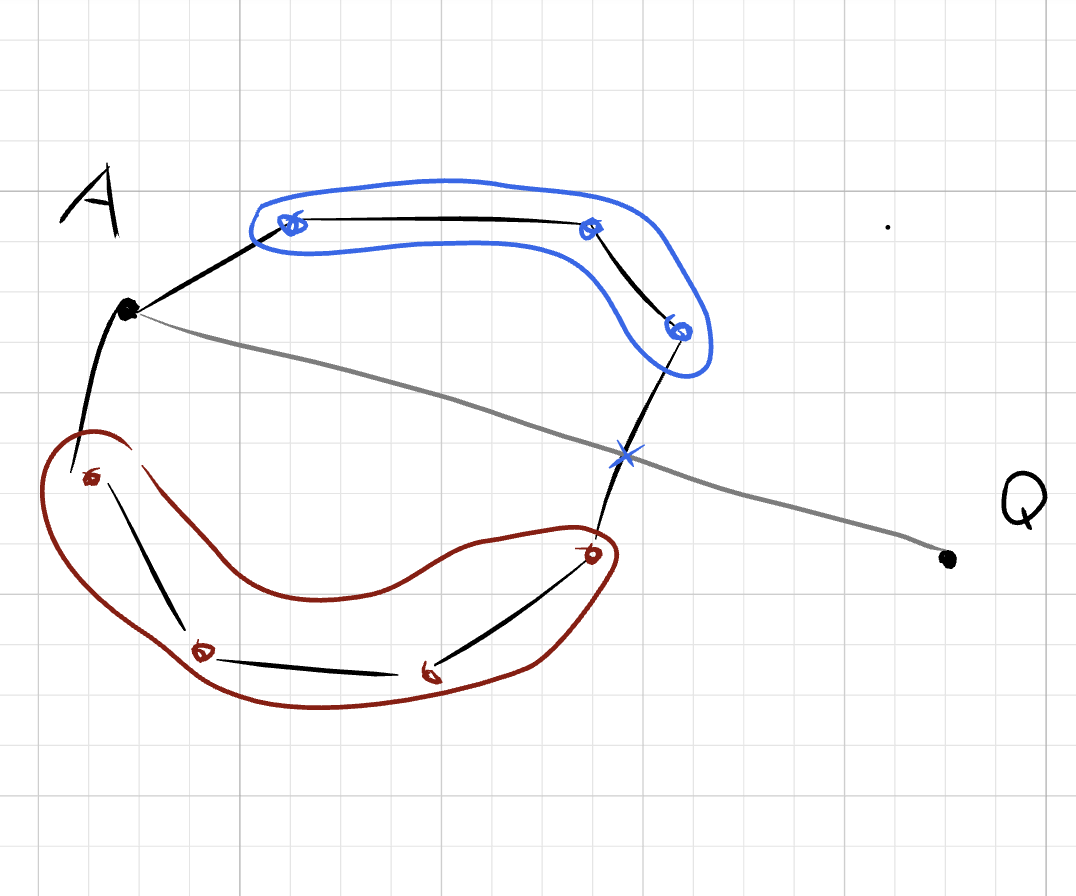
\includegraphics[width=\textwidth]{images/poly_splitted.png}
        \captionof{figure}{A - рандомная вершина, Q - точка запроса}
        \label{fig:Splitted_poly}
    \end{minipage}
    \hspace{0.05\textwidth}
    \begin{minipage}{0.5\textwidth}
        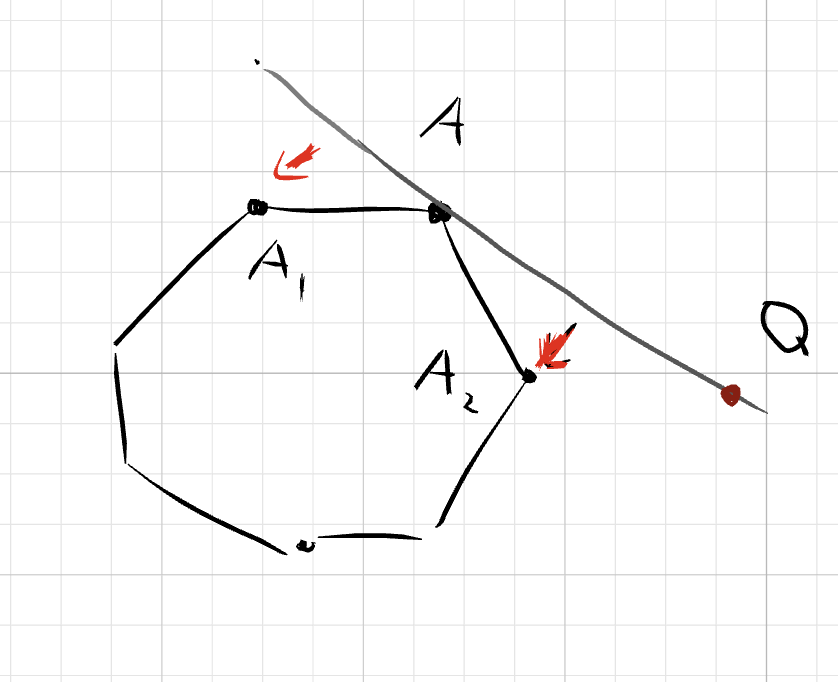
\includegraphics[width=\textwidth]{images/point_poly.png}
        \captionof{figure}{обе вершины $A_1, A_2$ находятся ниже прямой}
        \label{fig:Point_in_poly}
    \end{minipage}
\vspace{1cm}
\\
(I)Наша цель найти точку самую "Нижнюю" по углу от прямой QA против часовой, и самую "верхнюю" по часмовой. 
\autoref{fig:poly_in_lines}.\\
Для этого мы разделим наши вершины, на те которые сверху, и снизу нашей прямой AQ\footnote{заметим что они образуют отрзок точек если рассматривать массив точек отсортированых по часовому обходу}.\\
Делаем мы это для того чтобы можно было потом запустить тернарный поиск по самому "нижнему" углу в нижней части и по самоу "верхнему" углу в верхей части. Так как в разделенных частях вершины идут у нас в хорошем порядке, то есть вначеле возврастают по углу, а потом убывают(или наоборот в другой части). \autoref{fig:Monotonic_angle}\\
\noindent \begin{minipage}{0.5\textwidth}
    \vspace{1cm}
    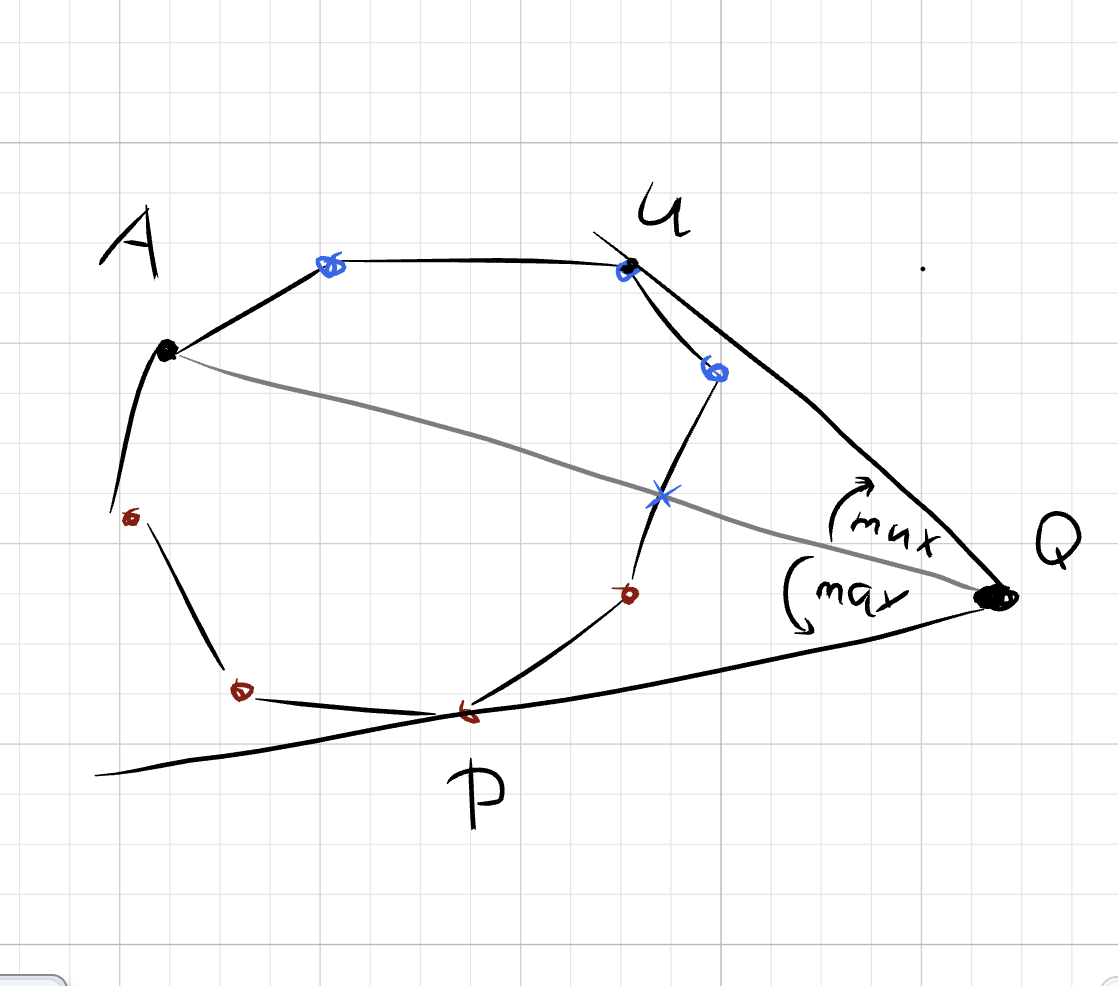
\includegraphics[width=\textwidth]{images/poly_in_lines.png}
    \captionof{figure}{U - кастальная сверху, D - касательная снизу\\max- здесь значит что max угол относительно QA, по-и против часой стрелке соотв.}
    \label{fig:poly_in_lines}
\end{minipage}
\hspace{0.05\textwidth}
\begin{minipage}{0.5\textwidth}
    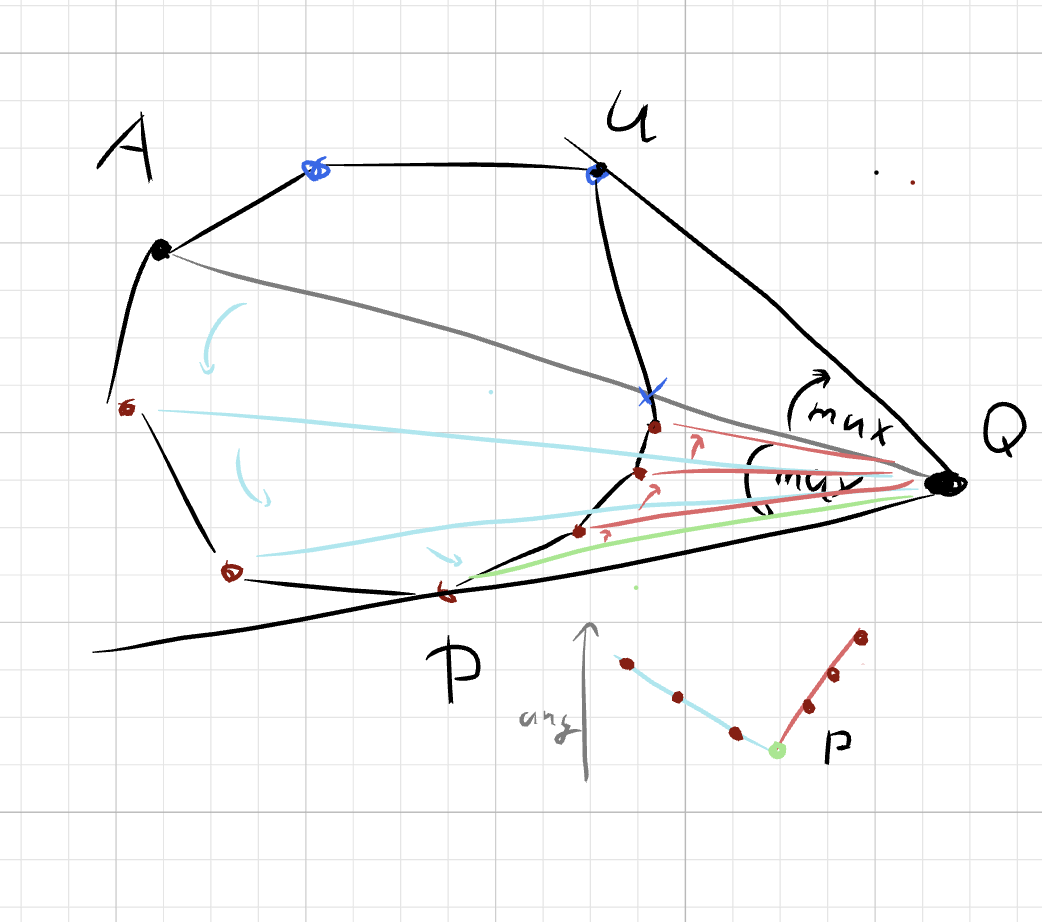
\includegraphics[width=\textwidth]{images/monotonic_angle.png}
    \captionof{figure}{Для нижней части угол вначале возврастает, потом убывает, снизу график угла}
    \label{fig:Monotonic_angle}
\end{minipage}
\vspace{1cm}

\emph{Опишем алгоритм} (I):\\
Пусть мы ищем нижнюю половину\footnote{для верхней симетричный алгос}. Пронумеруем, для удобства вершины начиная с вершины A, проитив часовой стрелки. Заметим теперь что вначале идут точке ниже, тоесть с положительнеым углом\footnote{положительным векторным произведением} относительно QA, а оптом с отрицательным углом, а значит можно запустить бинарный поиск, и найти точку разделяющюю положительный и отрицательный наклон\autoref{fig:splitting_point_poly}, она и будет определять конец отрезка вершин, которые снизу нашей прямой. Далее запускаем тернарный поиск по min/max углу в обеих частях\\
В случае когда мы угадали вершину касания, пронумеруем точки начиная с нашей по часовой стрелки, заметим что угол будет возврастать какой-то префикс, а потом убывать, а вторая вершина касания будет максимальная по углу вершина \autoref{fig:extra_case_poly}\\
\noindent \begin{minipage}{0.5\textwidth}
    \vspace{1cm}
    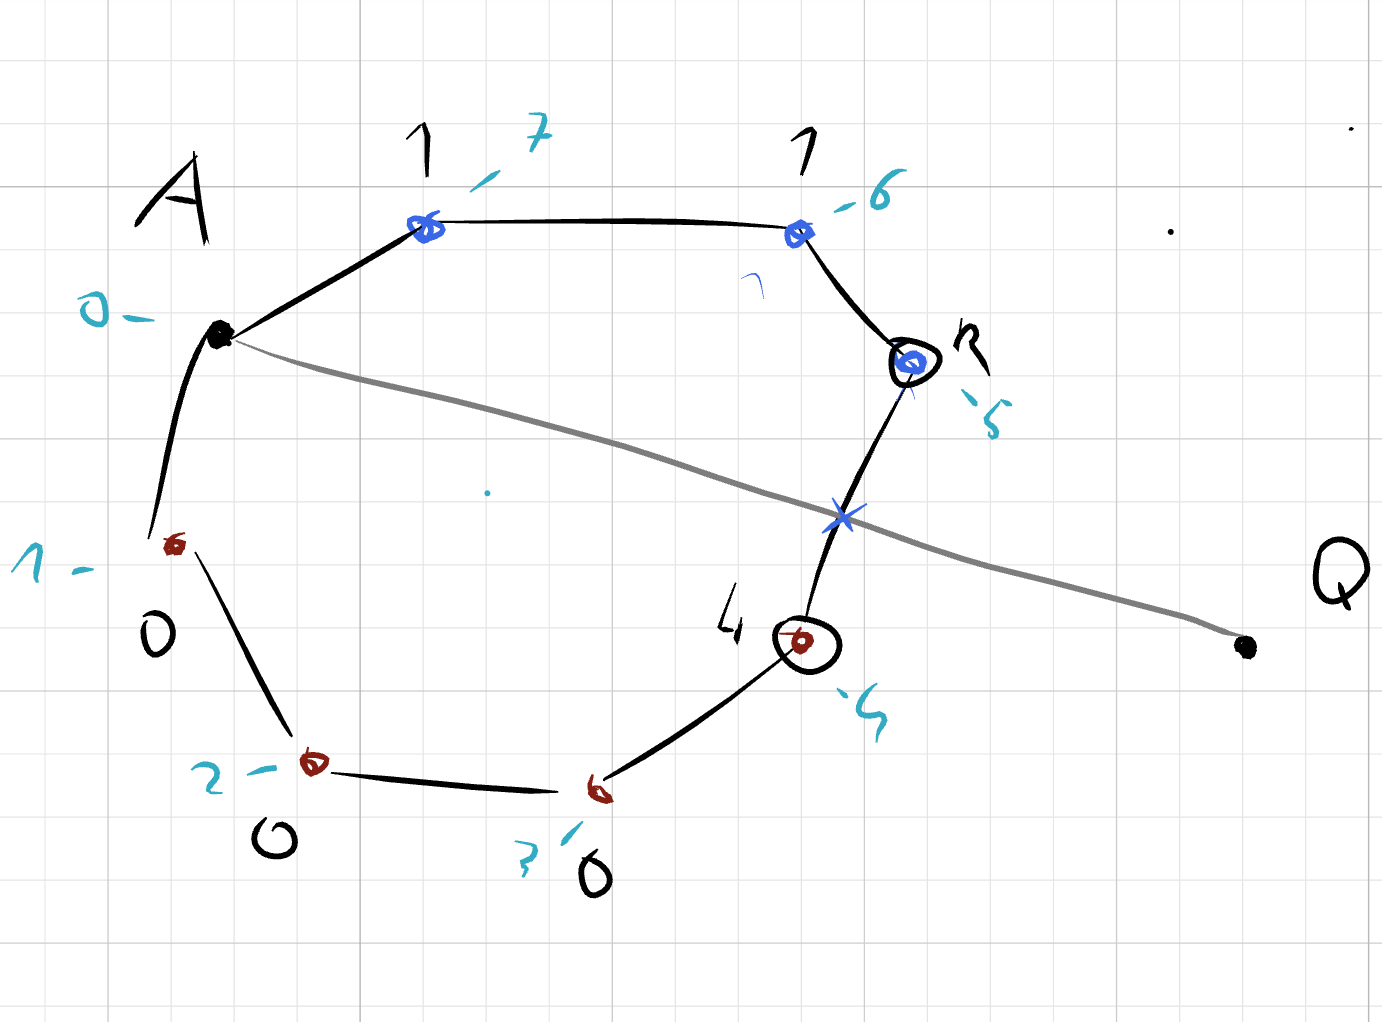
\includegraphics[width=\textwidth]{images/bs_splitting_point.png}
    \captionof{figure}{где L, R - границы бинарного поиска\\вначале они находятся в точках: 1, n-1}
    \label{fig:splitting_point_poly}
\end{minipage}
\hspace{0.05\textwidth}
\begin{minipage}{0.5\textwidth}
    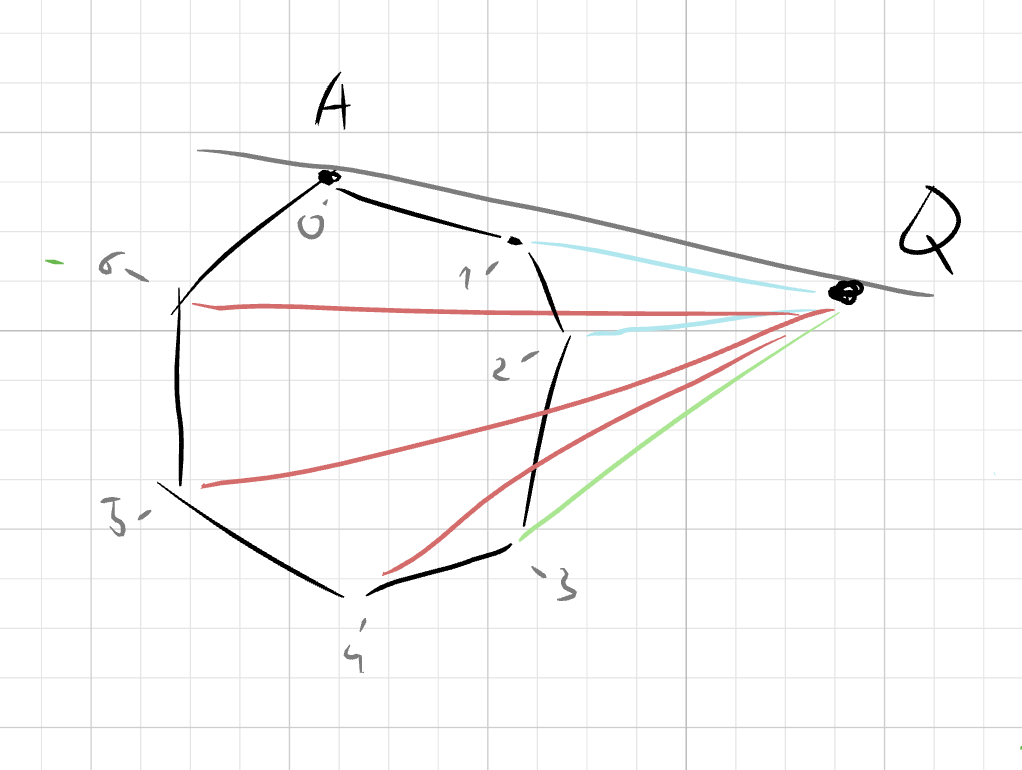
\includegraphics[width=\textwidth]{images/extra_case_poly.png}
    \captionof{figure}{пронумеровав вершины от A, получили точки которые возврастают, а потом убывают по углу}
    \label{fig:extra_case_poly}
\end{minipage}
\\
А вообще можно заметить что если взять произвольную точку на многоугольнике, и начать отчет от нее, то полярный угол будет вначале возврастать потом убывать потом снова возврастать, а на ней нужно нам найти min/max по углу точку как точки касания, последовательности такой "монотоности" называются битоническими, и на них можно запускать типа тернарного поиска, и не писать всю эту залупу.
\subsubsection*{Паралельные прямой:}
Заметим следующее свойство вершин,\\
которые являются врешинаси касательных, паралельной прямой:\\
Пусть вершина P - точка нижнего касания, тогда, точки A, B- вершины сосдение к P.\\
Проведем вектора AP, PB и отложим из точки P вектор соноправленый нашей прямой, пусть PQ.\\
Тогда получим что вектора AP, PB находятся по разные стороны от вектора PQ. \autoref{fig:poly_tagents_vec}\\
Однако же, для точек которые не являются касательными, вектора AP, PB будут находитмя по одну сторону\autoref{fig:poly_non_tagents_vec}.\\ Это доказывается тем фактом, что точка является точкой касания тогда и только тогда когда если мы проведем прямую через эту точку, соседние точки этой будут находмтся по одну сторону от прямой.\\
Так же замети что если взять стороны многоугольника, пускай ориентированы по часовой стрелке, то, в силу выпуклости, получим что они отсортированы по полярному углу\\
\noindent \begin{minipage}{0.5\textwidth}
    \vspace{1cm}
    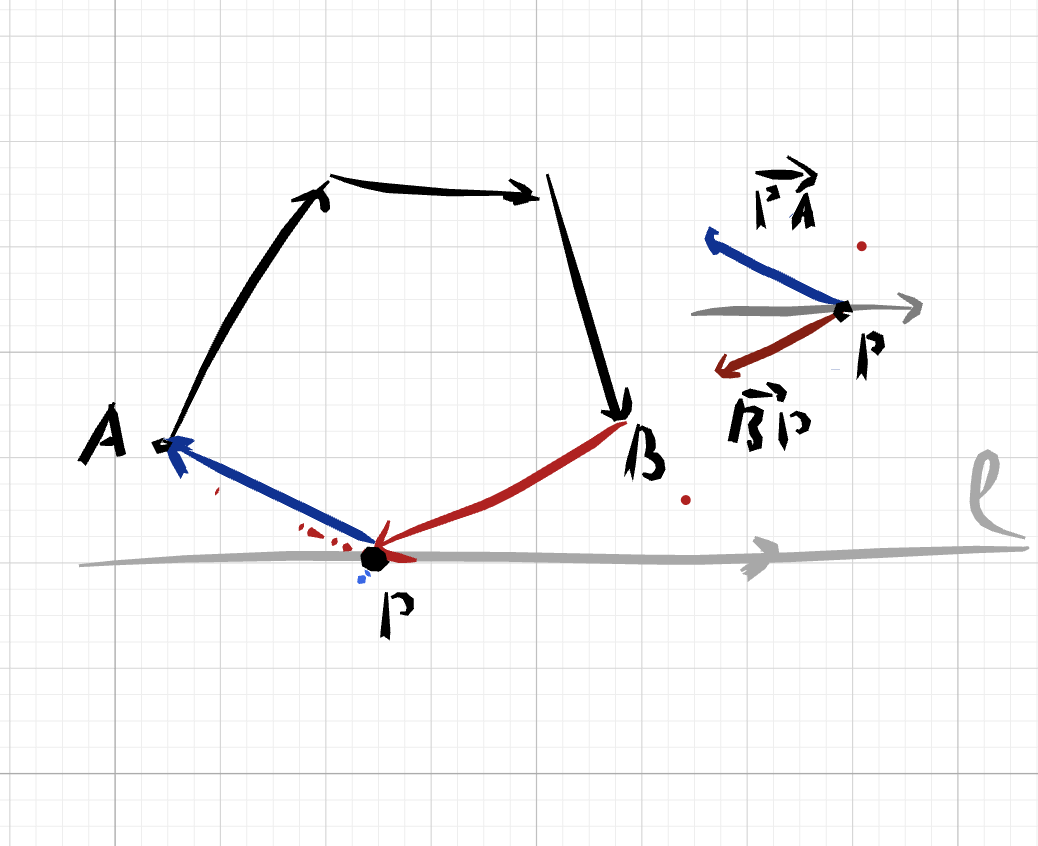
\includegraphics[width=\textwidth]{images/tangents_vec.png}
    \captionof{figure}{P- точка касания и ветора находятся по разные стороны от прямой}
    \label{fig:poly_tagents_vec}
\end{minipage}
\hspace{0.05\textwidth}
\begin{minipage}{0.5\textwidth}
    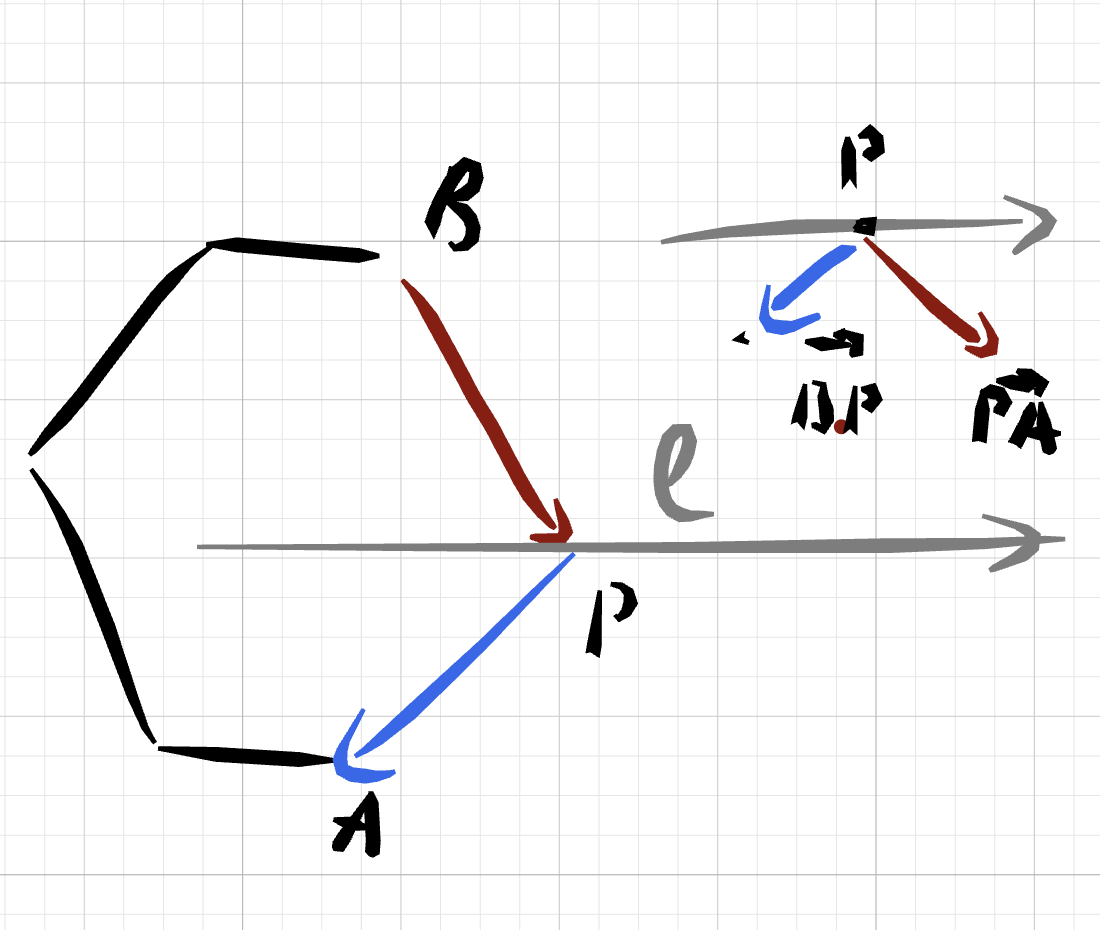
\includegraphics[width=\textwidth]{images/non_tangents_vec.png}
    \captionof{figure}{P - не точка касания и вектора находятся по одну сторону}
    \label{fig:poly_non_tagents_vec}
\end{minipage}
\vspace{1cm}\\
А значит, в силу предыдущих замечаний нам нужно найти две пары таких разделяющих векторов, которые находятся по разные стороны от прпямой. \autoref{fig:splitted_on_vevs}\\
Для этого достаточно запустить бинарный поиск который ищет место для двух, противоположныйх, векторов соноправленых прямой.\\
\emph{Примечание}Для бп нужен компоратор, пускай, мы сортируем пучек по полярному углу, от прямой, в деталях, мы сомтрим в какой полуплоскости от oX находится вектор, вектора находящие в верхей идут первыми, далее сравниваем угол относительно прямой oX, для одинакых плоскостей. Если вектор на oX, то если он напрвен вдоль, он идет самым первым, если противоположный, то идет в начале векторов нижней полуплоскости. \autoref{fig:polar_sort}\\
\noindent \begin{minipage}{0.5\textwidth}
    \vspace{1cm}
    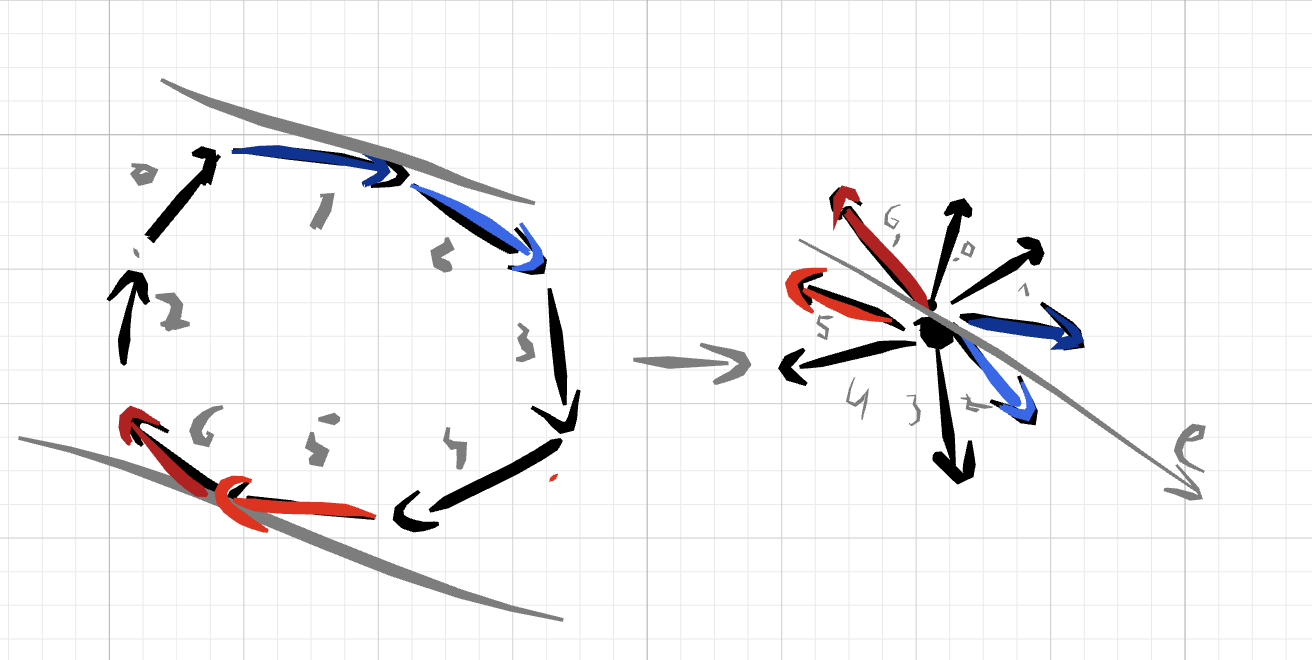
\includegraphics[width=\textwidth]{images/splitted_on_vecs.png}
    \captionof{figure}{Синие вектора найдутся бинарным поском для вектора соноправленому показаному вектору\\ Красные - для противоположно направленого}
    \label{fig:splitted_on_vevs}
\end{minipage}
\hspace{0.05\textwidth}
\begin{minipage}{0.5\textwidth}
    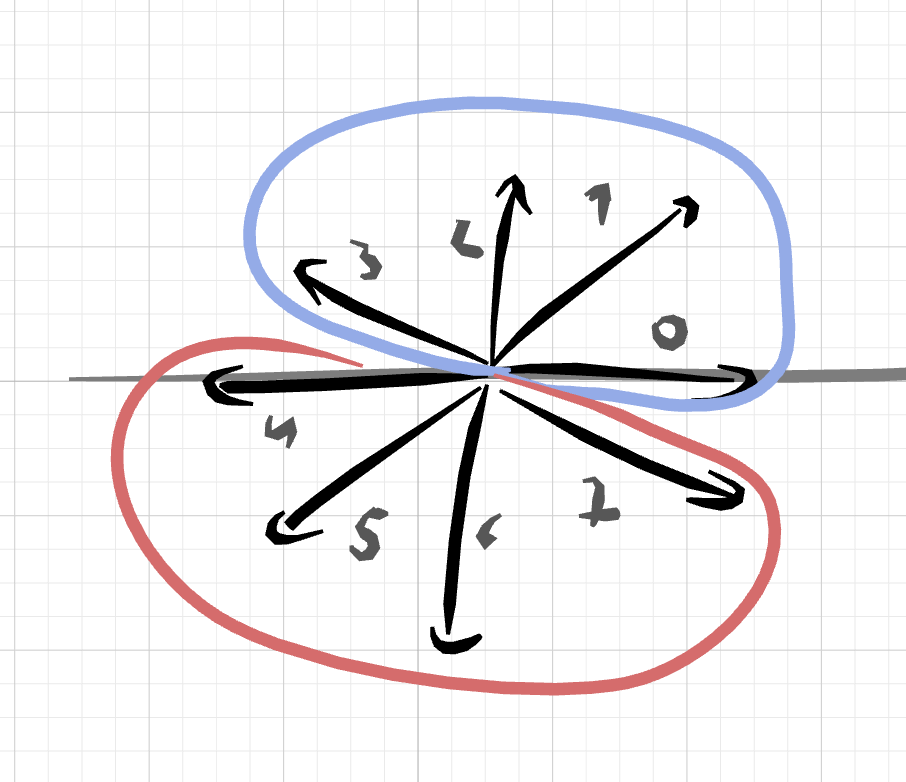
\includegraphics[width=\textwidth]{images/polar_sort.png}
    \captionof{figure}{}
    \label{fig:polar_sort}
\end{minipage}
\vspace{1cm}\\
\subsubsection*{Пересечение с прямой:}
Эта задача тесно связана с предыдущей, нам нужно найти точки касания, далее разбить наш многоугольник на части относительно касательных\autoref{fig:splitted_by_tangents}, а далее, так как двух пловинах оринтированое растояние точек, до данной прямой будет монотонно убывать/возврастать\autoref{fig:bin_search_distance_poly} то можно запустить бинарный поиск.\\
\noindent \begin{minipage}{0.5\textwidth}
    \vspace{1cm}
    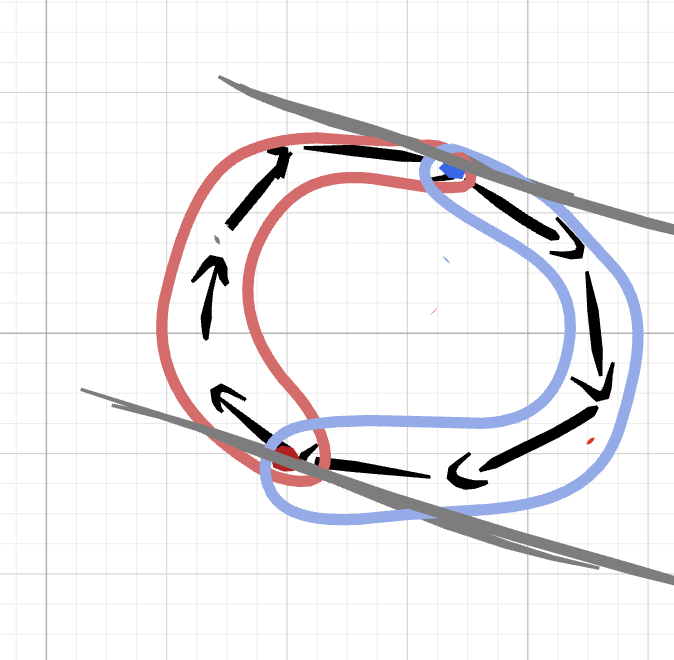
\includegraphics[width=\textwidth]{images/splitted_by_tangents.png}
    \captionof{figure}{}
    \label{fig:splitted_by_tangents}
\end{minipage}
\hspace{0.05\textwidth}
\begin{minipage}{0.5\textwidth}
    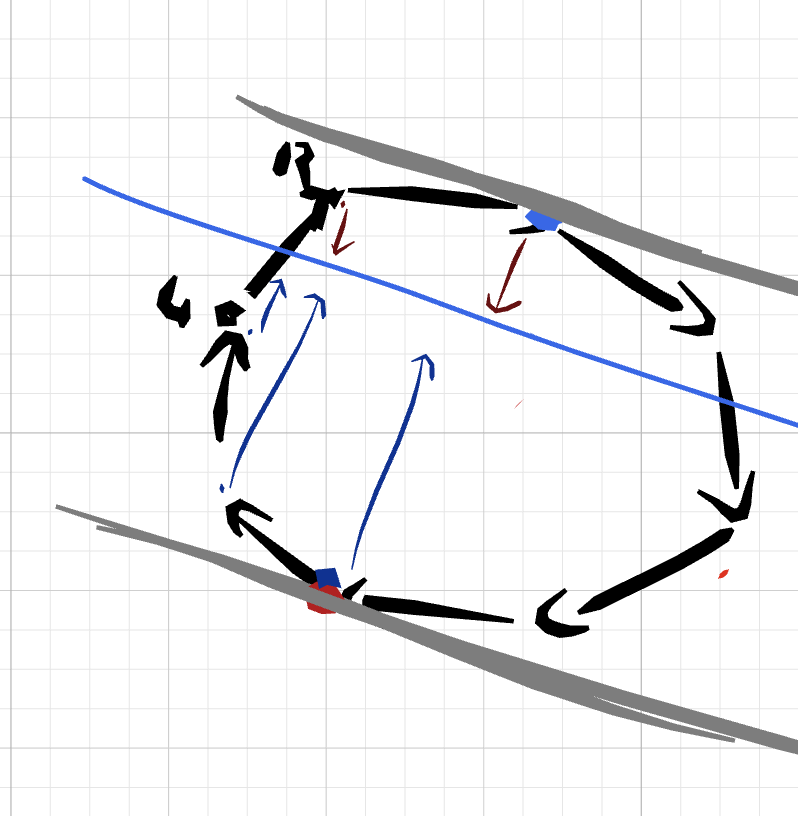
\includegraphics[width=\textwidth]{images/bin_search_distance_poly.png}
    \captionof{figure}{где синие стрелки-отрицательно ор. растояние, красные-положительное,\\ L,R итоговые границы бинарного поиска для левой половины многоугольника}
    \label{fig:bin_search_distance_poly}
\end{minipage}
\vspace{1cm}\\
\subsection*{Сумма Минковского}
\subsubsection*{Доказательство выпуклости суммы выпуклых}
\emph{Определение выпуклости}: A - выпуклое мн-во $\Leftrightarrow \forall p, q \in A: p \cdot \lambda + q \cdot (1 - \lambda) | \forall \lambda \in [0, 1]$\\
Пусть x, y - точки суммы Минковского: $x, y \in A$\\
Тогда эти точки расскладываются на суммы точек из других фигур:\\
$x = p_1 + q_1$, $y = p_2 + q_2$, $|p_1, p_2 \in P, q_1, q_2 \in Q$.\\
Теперь проверим критерий выпуклости сформулированый выше:
\begin{multline*}
    a = x \cdot \lambda + y \cdot (1 - \lambda) = (p_1 + q_1) \cdot \lambda + (p_2 + q_2) \cdot (1 - \lambda) = p_1\lambda + q_1\lambda + p_2(1 - \lambda) + q_2(1 - \lambda) =\\
    = (p_1\lambda + p_2(1 - \lambda)) + (q_1\lambda + q_2(1 - \lambda)) = [p'=p_1\lambda + p_2(1-\lambda) \in P \text{(так как P, Q - выпуклы)}] = p' + q'\\
    p' \in P, q' \in Q \Rightarrow a \in A
\end{multline*}
\subsubsection*{Доказательство того что у нас получится многоугольник\footnote{выпуклой фигурой может быть, например, круг}}
Я докажу больше, что: $X \oplus Y = conv(\sum_{i,j} x_i + y_j) | x_i \in X, y_j \in Y$\\
\begin{proof}[доказательство $conv(\sum_{i,j} x_i + y_j) \subseteq X \oplus Y$:] тут просто\\
    Мы знаем что любая вершина $x_i + y_j \in X \oplus Y$\footnote{так как $x_i \in X, y_i \in Y$ и определению суммы}\\
    А еще мы знаем что сумма это фигура-выпукла следовательно стороны тоже принадлежат сумме. \autoref{fig:edge_in_sum_mekovski}\\
    Стороны принадлежат сумме следовательно если взять "крайние" то есть как раз те которые приндлежат выпуклой оболочке стороны, и снова вспомнить про выпуклость фигуры, то получим что и внутрености сторон тоже принадлежат сумме.
\end{proof}
\begin{proof}[доказательство $conv(\sum_{i,j} x_i + y_j) \supseteq X \oplus Y$] тут повозиться надо\\
    возьмем произвольную точку $a \in X \oplus Y$ разложим ее на сумму $a = x' + y' | x' \in X, y' \in Y$\\
    Треангулируем X, Y, так как известно что они выпуклые многоугольники. \autoref{fig:tri_sum_menkovski}\\
    Находим $x_1, x_2, x_3 \in X$ - треугольник, которому принадлежит $x' \in (x_1, x_2, x_3)$\\
    Находим $y_1, y_2, y_3 \in Y$ - треугольник, которому принадлежит $Y' \in (y_1, y_2, y_3)$\\
    $x', y'$ можно задать координатами треугольников $(x_1, x_2, x_3), (y_1, y_2, y_3)$:\\
    $x' = x_1 \cdot \alpha_1 + x_2 \cdot \alpha_2 + x_3 \cdot \alpha_3 | \alpha_1 + \alpha_2 + \alpha_3 = 1$\\
    $y' = y_1 \cdot \mu_1 + y_2 \cdot \mu_2 + y_3 \cdot \mu_3 | \mu_1 + \mu_2 + \mu_3 = 1$\\
    поэтапно построим точку $a$:\\
    Возьмем минимальный из коофицентов $\mu_1, \alpha_1$, пусть $\mu_1$ тогда вычтем из a: $x_1 \mu_1 + y_1 \mu_1$\\
    Получаем:\\
    $a = (x_1 + y_1) \cdot \mu_1 + a' = (x_1 + y_1) \cdot \mu_1 + x'' + y''$\\
    $x'' = x_1 \cdot (\alpha_1 - \mu_1) + x_2 \cdot \alpha_2 + x_3 \cdot \alpha_3 | \alpha_1 + \alpha_2 + \alpha_3 = 1 - \mu_1$\\
    $y'' = y_2 \cdot \mu_2 + y_3 \cdot \mu_3 | \mu_1 + \mu_2 + \mu_3 = 1 - \mu_1$\\
    Снова возбмем минимум, из первых переменных: $(\alpha_1 - \mu_1)$ и $\mu_2$, пусть $\mu_2$\\
    $a = (x_1 + y_1) \cdot \mu_1 + (x_1 + y_2) \cdot \mu_2 + a''$\\
    Так далее пока не получим разбиение:\\
    $a = (x_{i_1} + y_{j_1}) \cdot \alpha_1 + (x_{i_2} + y_{j_2}) \cdot \alpha_2 + (x_{i_3} + y_{j_3}) \cdot \alpha_3 + ... + (x_{i_k} + y_{j_k}) \cdot \alpha_k | \alpha_1 + ... + \alpha_k = 1$\\
    Напомню, что для доказательства обратного вложение, нужно доказать что:\\
    точка $a \in X \oplus Y$ принадлежит также $conv(\sum_{i, j} x_i + y_j)$, мы получили выше разложение, это задание точки a, в виде координат вершин многоугольника с некоторыми вершинами $x_{i_t}, y_{j_t} \in conv(\sum_{i, j} x_i + y_j)$. conv - выпукла, следовательно любая точка, которая является комбинацией ее вершин с коофицентами в сумме дающие 1. В частности принадлежит и т. a
\end{proof}
\noindent \begin{minipage}{0.3\textwidth}
    \vspace{1cm}
    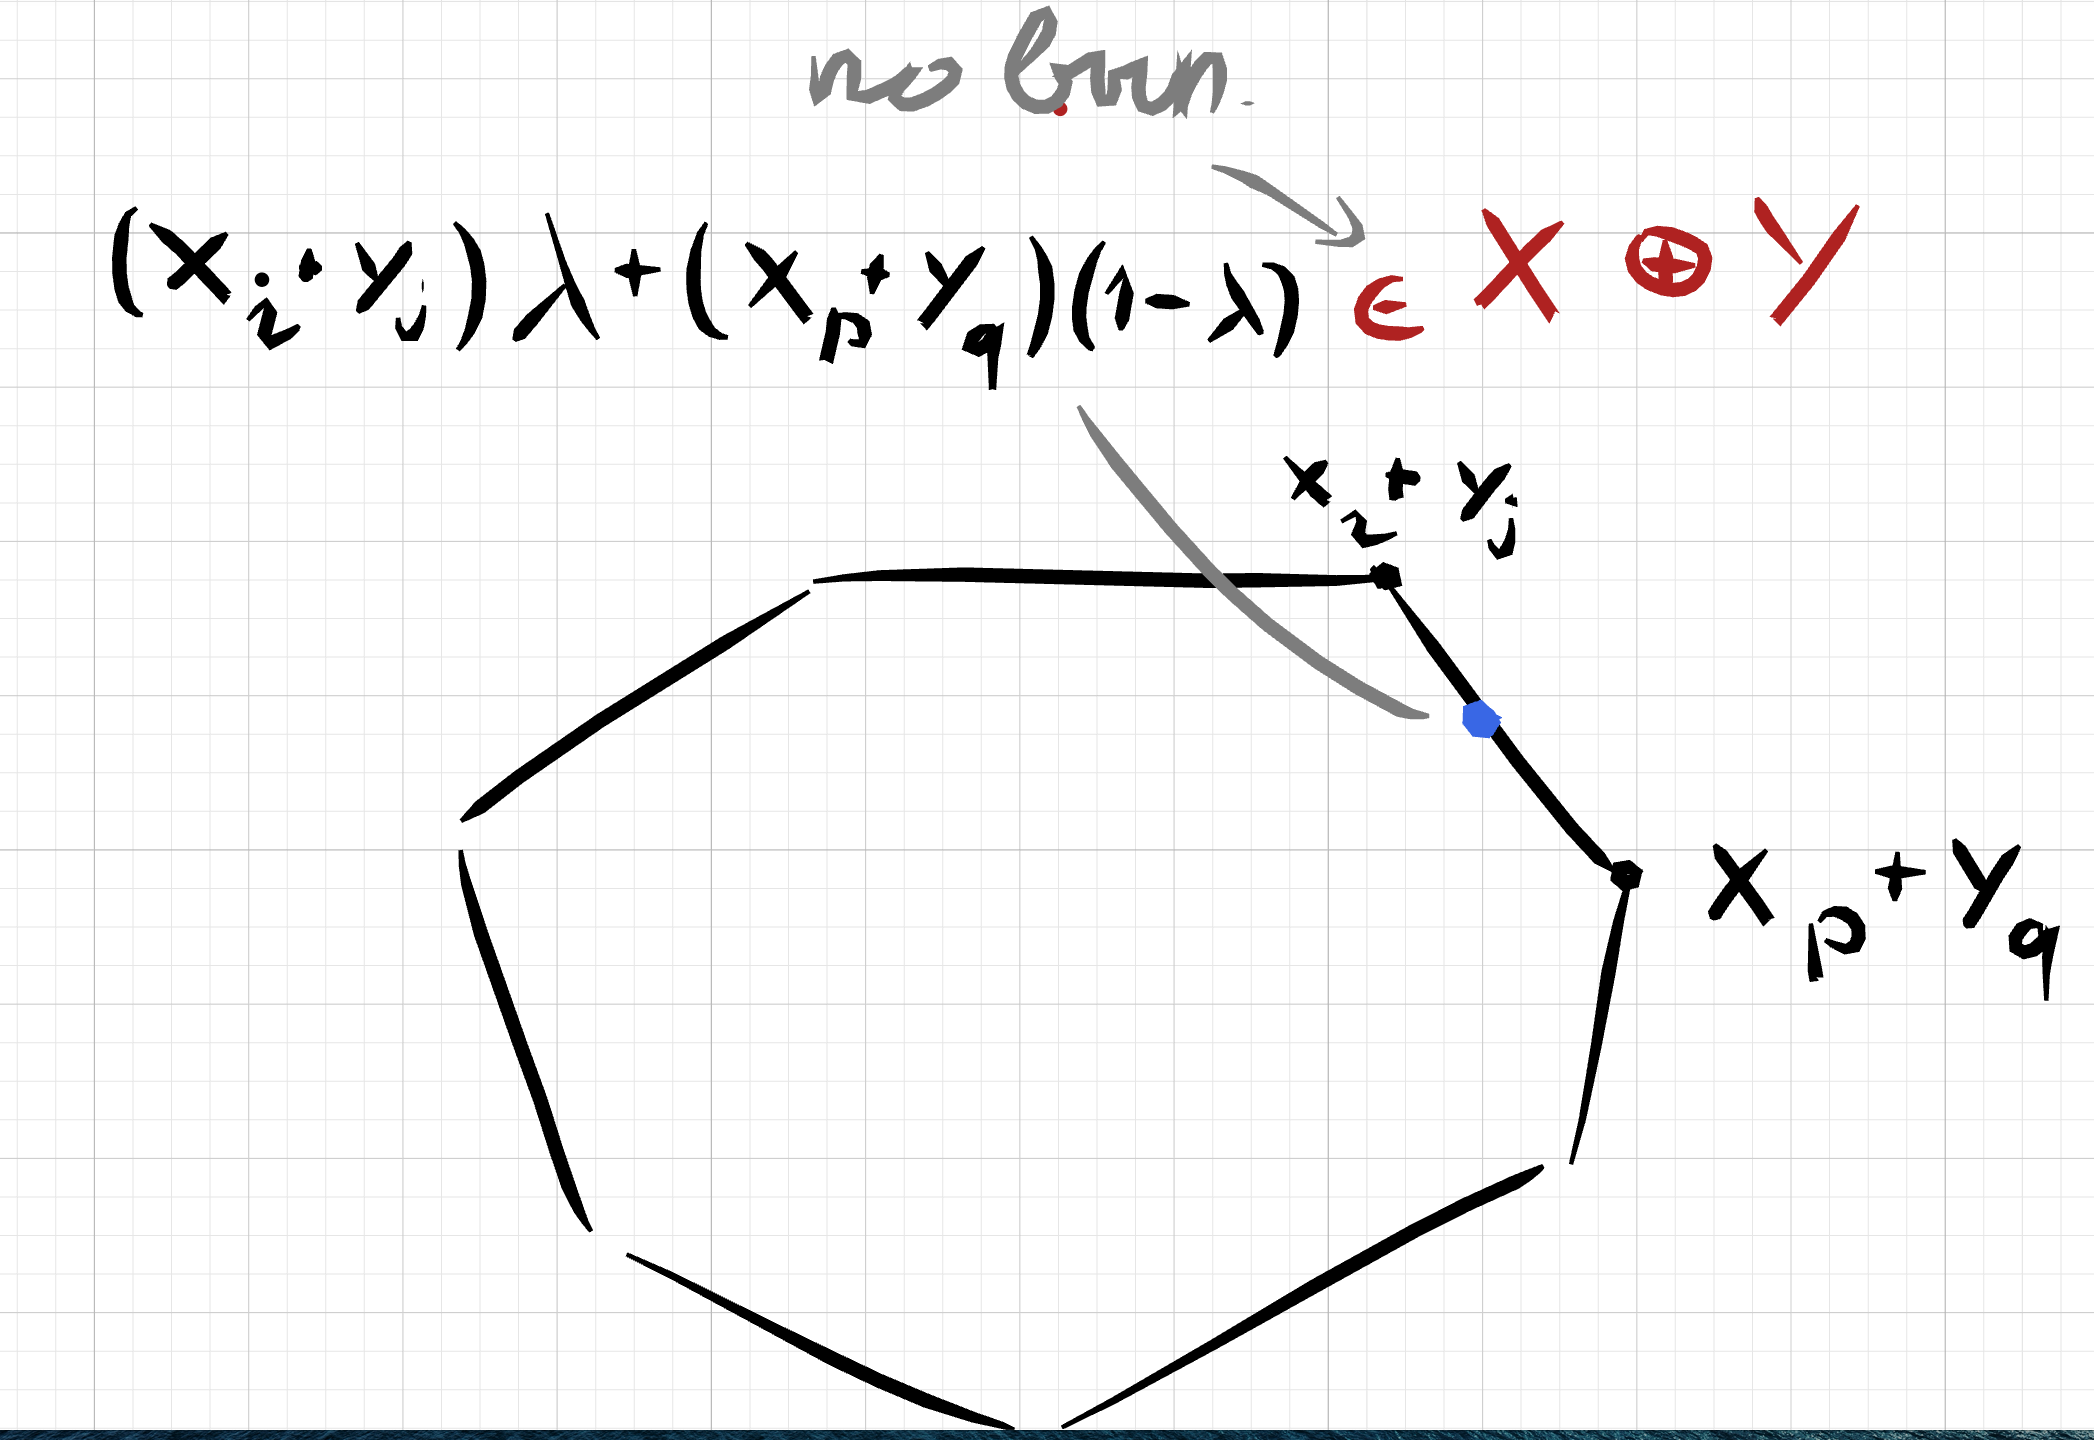
\includegraphics[width=\textwidth]{images/sum_menk_edge.png}
    \captionof{figure}{}
    \label{fig:edge_in_sum_mekovski}
\end{minipage}
\hspace{0.1\textwidth}
\begin{minipage}{0.3\textwidth}
    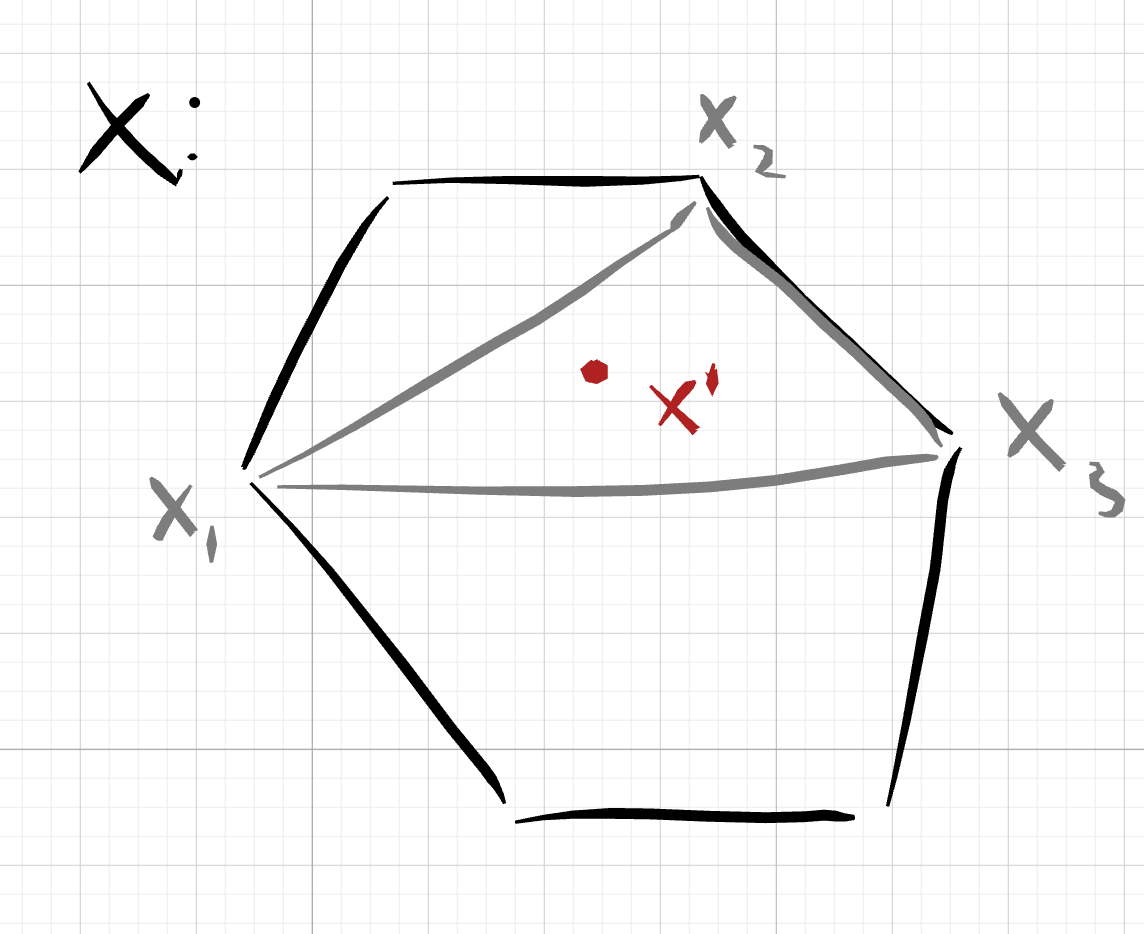
\includegraphics[width=\textwidth]{images/tri_sum_menk.png}
    \captionof{figure}{}
    \label{fig:tri_sum_menkovski}
\end{minipage}
\subsubsection*{Доказательство что сторона суммы, это сторона одного из исходных}
Возьмем сторону $AB \in X \oplus Y$, возьмем прямую $l \perp AB$\\
Сделаем на нее проекцию многоугольника. \autoref{fig:projector_menkovski}.\\
Заметим что в рассматривоемой проекции наша сторона перейдет в крайнюю точку на прямой $A'$.\\
Теперь рассмотрим и проекции сторон исходных многоугольников $X, Y$. Так как в проекци сумма переходит тоже в сумму, то получаем что не может быть в X, Y точки которая крайнее $A'$.\\
А также что хотя бы в одном многоугольнике должна найтись точка такая что уходит по проекции также в $A'$ \autoref{fig:XY_projector_menk}\\
\noindent \begin{minipage}{0.4\textwidth}
    \vspace{1cm}
    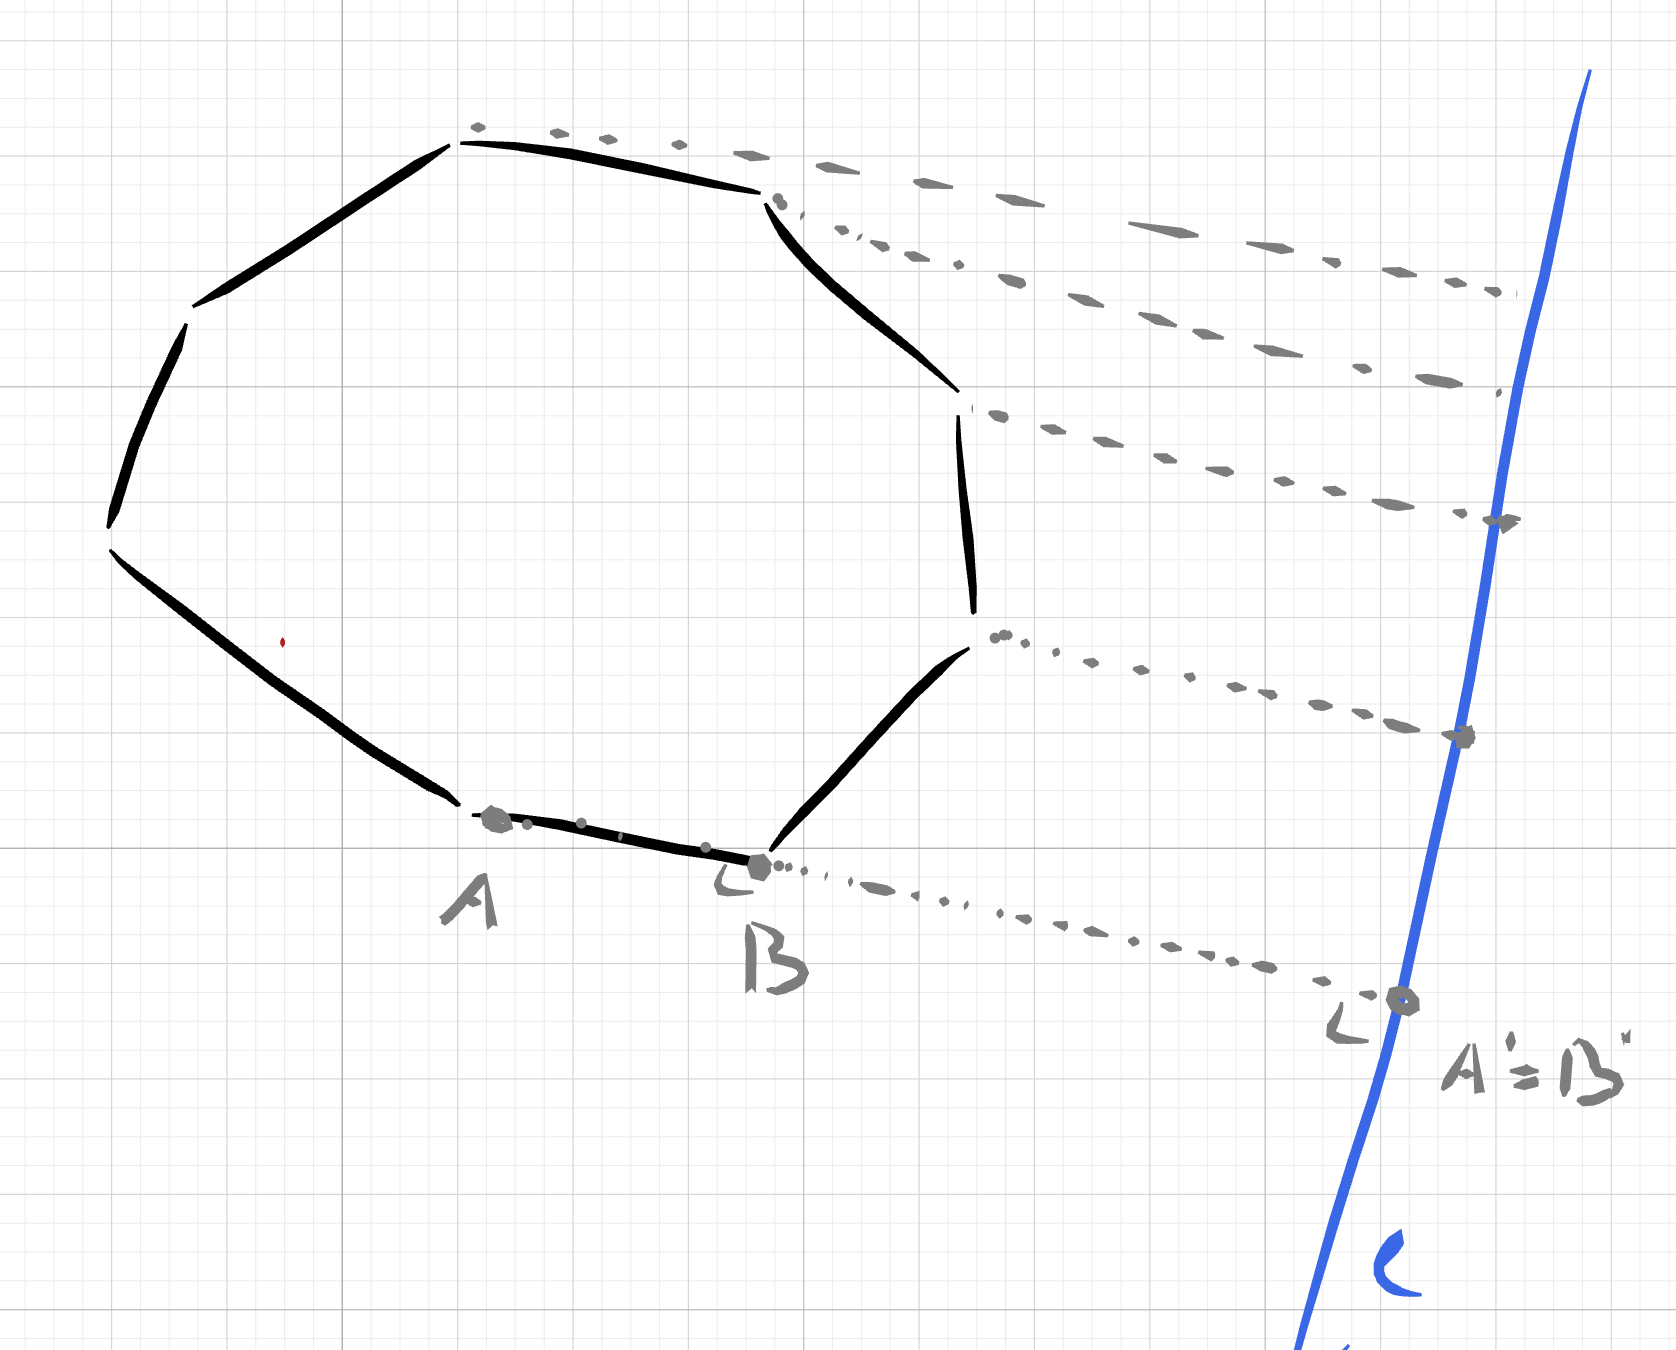
\includegraphics[width=\textwidth]{images/projector_menk.png}
    \captionof{figure}{}
    \label{fig:projector_menkovski}
\end{minipage}
\hspace{0.1\textwidth}
\begin{minipage}{0.4\textwidth}
    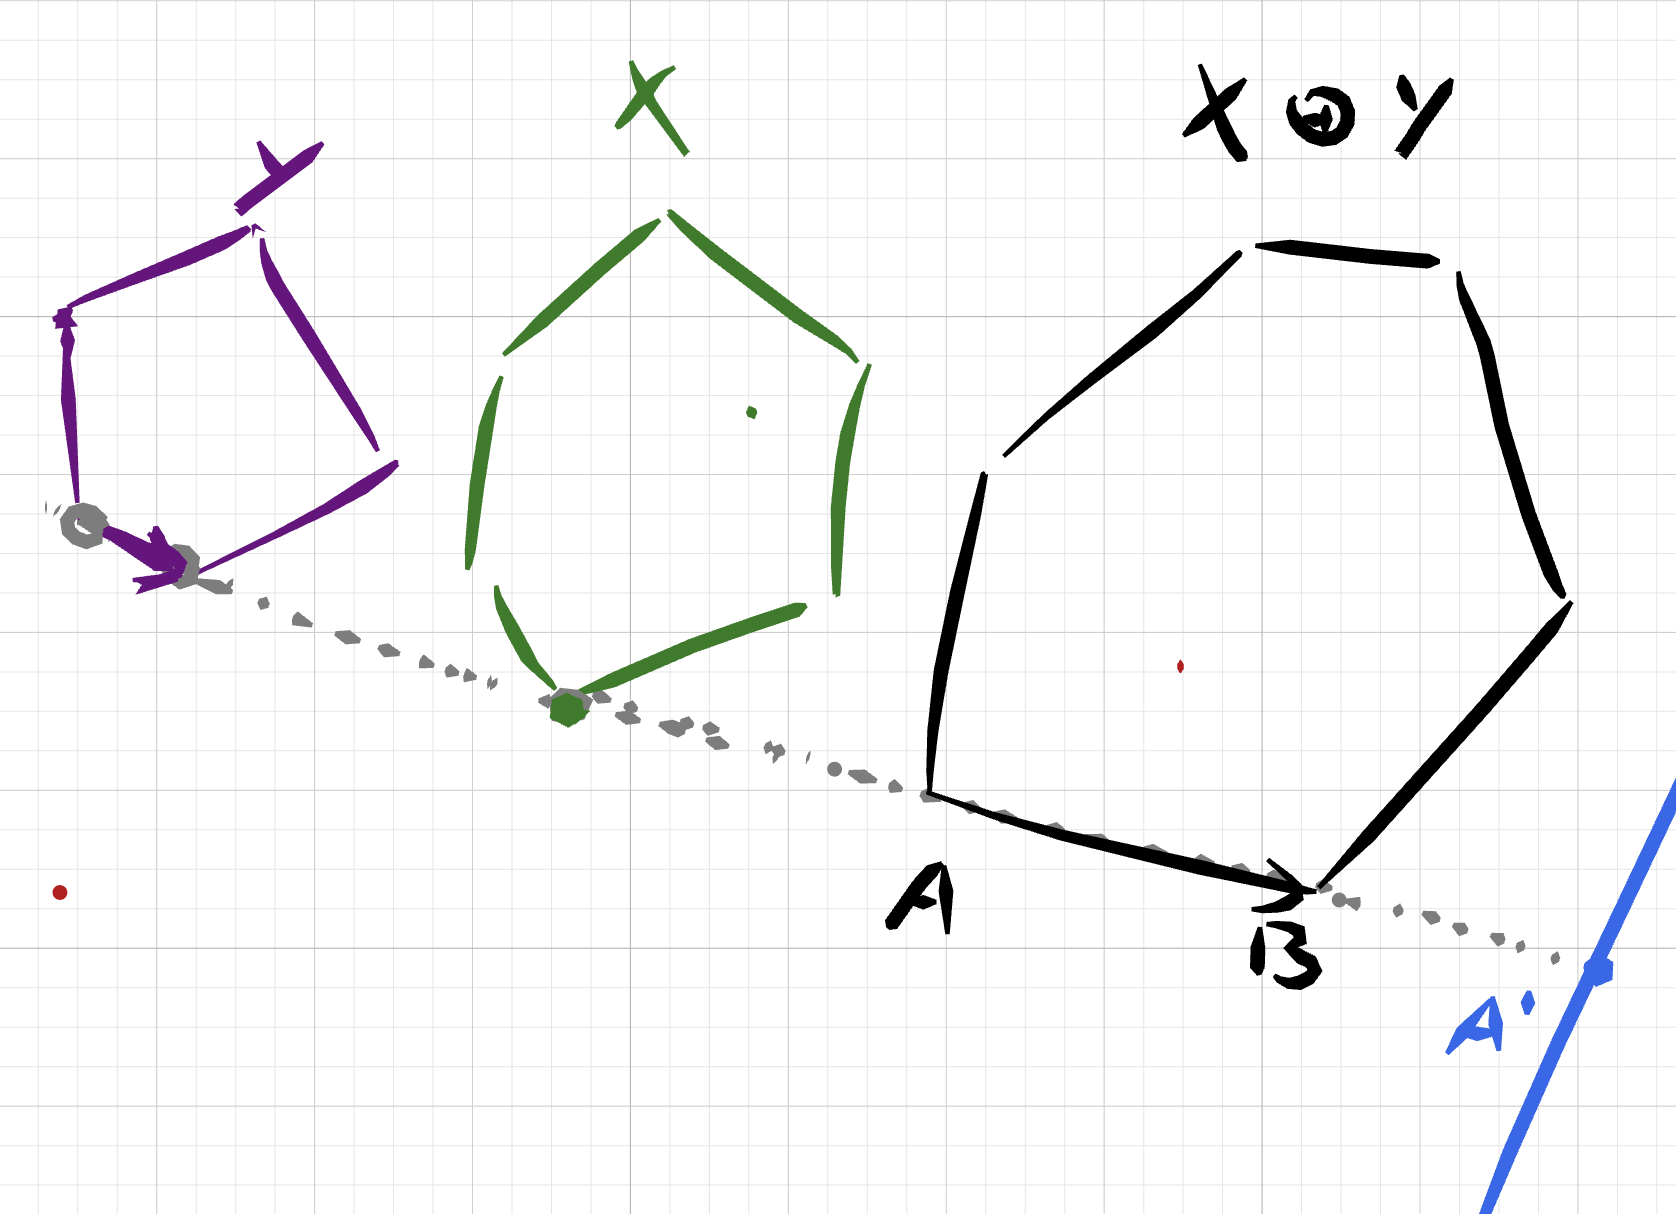
\includegraphics[width=\textwidth]{images/XY_projector_menk.png}
    \captionof{figure}{вообще говоря что стороны X, Y или точки находятся на одной и той же прямой не правда, но будем считать что мы сдвинули наши многоугольники чтобы так было, не умаляя общности так как мы пользуемся только крайностью}
    \label{fig:XY_projector_menk}
\end{minipage}
\vspace{1cm}\\
А так же мы знаем что AB - это отрезок, не точка, а следовательно из соображений что:\\
1)точка + точка = точка\\
2)и так как у нас в обоих фигурах A' - тоже крайняя\\
(либо многоугольник не доходит до перпендикуляра из A') следует что области которые будут переходить в $A'$ это либо отрезки либо точки\\
Получаем что $A'$ могла быть получена:\\
Либо комбинацией двух отрезов, либо одного отрезка из $X$ либо $Y$.\\
А следовательно сторона суммы - это сторона одного из исходных.\\
Что и требовалось\footnote{рассмотр проекции необходим для того чтобы ввести понятие "крайных" точек и не возиться с областями не похожими на отрезок или точку}
\subsubsection*{Доказательство что каждая сторона из X, Y присутсвует в сумме}
Этого я не нашел в доказательствах, но кажется это нужно доказывать, для алгоритма ниже.\\
Пускай у нас не встречается некоторая сторона, тогда рассмотрим такую же проекцию как и в предыдущем доказательстве, перепендекулярную стороне, мы получили что сторона спроектировалась в точку, она будет крайней, разберем так же крайнюю точку в сумме, так как рассматривоемой стороны нет в полученой сумме то крайняя точка получилась в результате проекции вершины, так как эта вершина суммы крайняя она должна была быть получена суммой крайних точек $x, y \in X, Y$, однако в одном из этих многоугольников крайняя точка-это проекция стороны, а значит и сумме должна получиться хотя бы сторона.
\subsubsection*{Алгоритм}
Из предыдущих фактов получаем алгоритм:\\
Взять все стороны обоих многоугольников, как вектора, допустим ориентированы по часовой. Мы знаем что любой вектор должен присутсвовать в сумме, и что любая сторона суммы это сторона многоульника. Значит, любая сторона была получена путем отложения от вершины, вектора одной из сторон многоугольников $X,Y$, любая сторона присутсвовала по факту выше, а значит в процессе должны использроваться все вектора.\\
Так же полученая сумма выпуклая, что задает нам порядок отложения векторов, по или против часовой стрелки\footnote{иначе получим не выпуклый многоугольник}.\\
Таким образом получаем алгоритм: взяли все вектора сторон по часовой стрелке, и начали откладывать их друг после друга, начинаясь c нижней левой точки, и порядок отложения будет по полярному углу, так что бы начальная точка была нижней левой\footnote{то есть откладывая вначале те вектора которые идут сразу после векторов направленых в нижнюю полуплоскость, если паралельных oX, то после направленых влево. Иначе отложим мы от начальной точки тот вектор который ведет вниз, или паралельно влево, что сломает наш инвариант про нижнюю левую точку}
\subsection*{Поиск пары пересекающих отрезков}
Такой метод называется \emph{Sweep line}.\\
Снизу будет приведен метод поиска всего одной пары.\\
Для общего случая ассимтотика будет $O((n + m)log(n))$ где m - кол-во пересечений.\\
Будем мысленно двигать вертикальную прямую слева на cправа, по мере движения будем добавлять и удалять отрезки, так чтобы их относительный порядок был по возврастанию y - координат пересечения с прямой.\footnote{Например, используя двоичное дерево.}\\
\emph{Замечания}:\\
\begin{itemize}
    \item Относительный порядок, относительно других отрезков, по мере движения вертикальной прямой, мог измениться если и только если отрезок с кем то пересекается \autoref{fig:crossing_segments}\\
    А следовательно пока мы не встертили пересечение отрезков, в относительный порядок не будет меняться.
    \item Пересекающие отрезки, когда-нибудь для некоторого $x$ будут рядом в относительном порядке по пересечению с вертикальной прямой, причем до пересечения!\autoref{fig:crossing_segments_near}
    Следовательно мы сократили колличество кандитов на пару пересечения с $n^2$ до $n$. Подробнее будет расписано ниже.
\end{itemize}
\noindent \begin{minipage}{0.3\textwidth}
    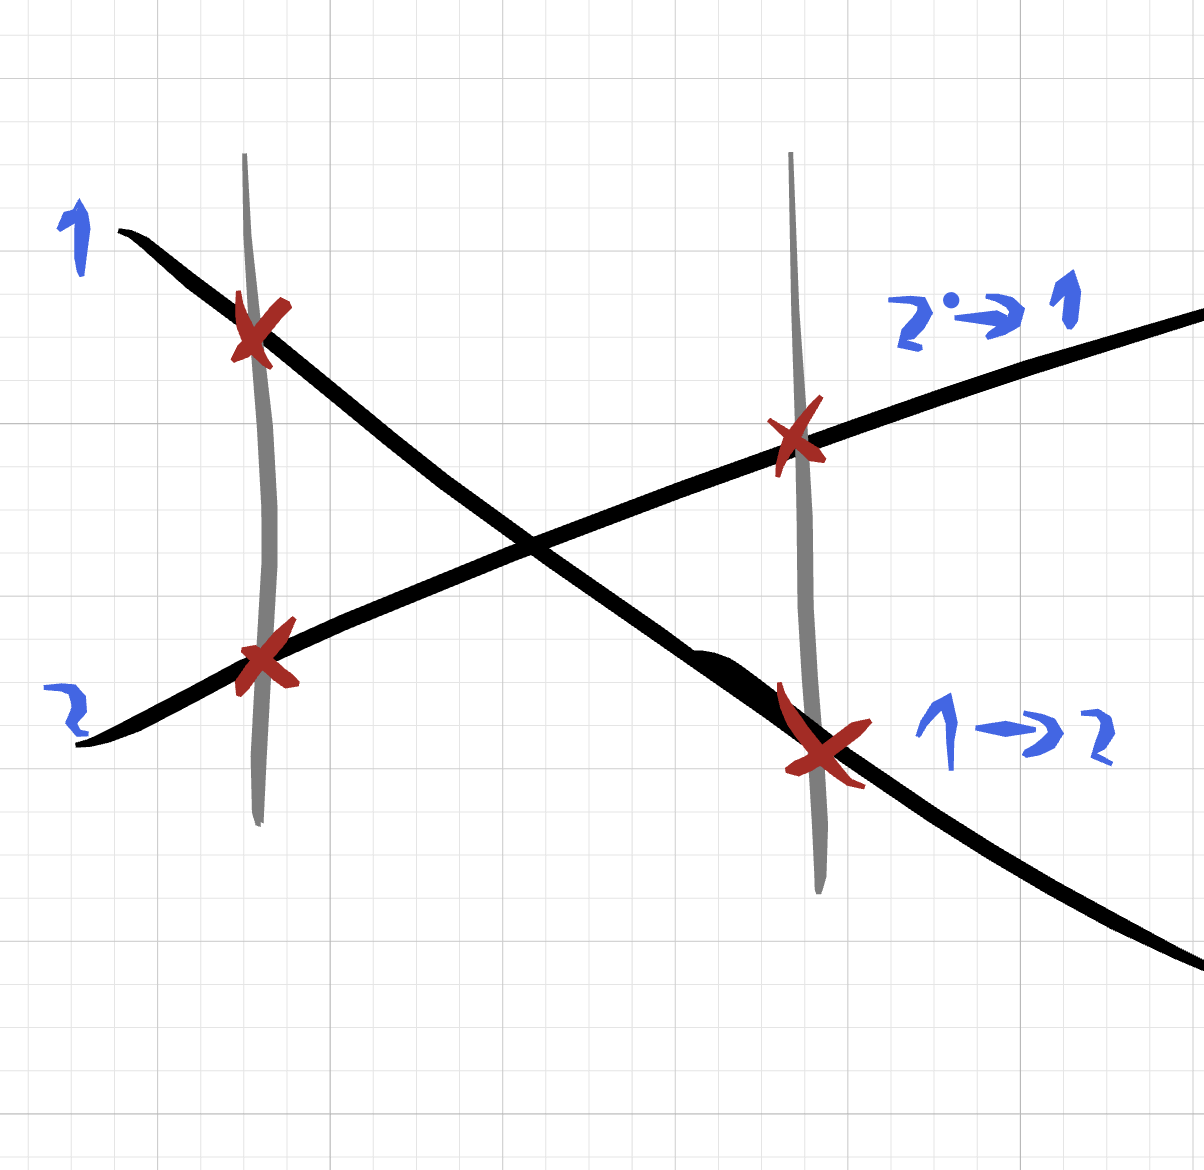
\includegraphics[width=\textwidth]{images/intersect_order_change.png}
    \captionof{figure}{}
    \label{fig:crossing_segments}
\end{minipage}
\hspace{0.1\textwidth}
\begin{minipage}{0.3\textwidth}
    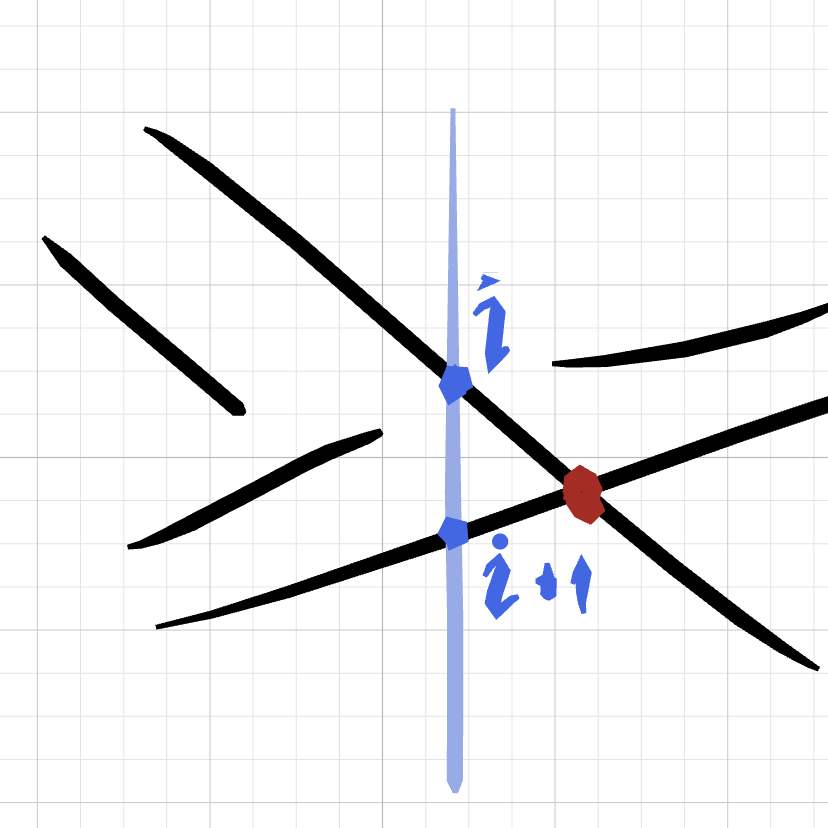
\includegraphics[width=\textwidth]{images/intersect_order.png}
    \captionof{figure}{}
    \label{fig:crossing_segments_near}
\end{minipage}
\vspace{1cm}\\
\emph{Алгоритм}:\\
В упрощеной задаче только с нахождением одной пары отрезков, мы будем поддерживать всего два события:
\begin{itemize}
    \item Отрезок начал пересекаться с заметающей вертикальной прямой
    \item Отрезок перестал пересекаться с заметающей вертикальной прямой
\end{itemize}
А проверять мы на пересечение пару будем только пару сосдних которая появляется при событиях выше. Этого будет достаточно, так как как сказано выше порядок не может поменяться перед тем как отрезки переклись, а мы предпологаем что отрезки не пересекались до данной позции\footnote{мы пользуемся что узнаем о пересечении отрезков до того как прямая дойдет до точки из пересечения, это правда так как отрезки окажутся соседними до пересечения}, а тогда соседние могут появлиться только при добавлении/удалении
\end{document}